\subsection{Required Resources \& Subsystem Responsibilities}

Description of the estimated resources need to carry out this implementation plan and what the roles and responsibilities are for each subsystem in this context.

Need to take information from Storage View subsections, then find gaps to confirm add with DWG or identify potential gaps for project/departments/groups to consider.

The departments and technical groups are responsible; documentation specialists primary assistants; and both depend on system administrators and software developers on case-by-case need.
Transition Joint Work.

\begin{enumerate}
	\item Documentation Quantification
	\item Documentation Selection
	\item Proposed repositories Reviewing
	\item Starting and Finishing Scheduling
\end{enumerate}

Recommend new Operations Documentation Committee/Group for project-wide support, common tools and distributed development of them, lessons learned, etc.
Project-provided charge and scope.
Composition: documentation lead(s), documentation specialists, SQuaRE seat, ex-officio manager (department or subgroup?)
Need Chuck, Austin, Leanne input to min (and possibly max) bound level of effort for this role.

\begin{figure}[t]
\caption{Temporary Caption.}
\centering
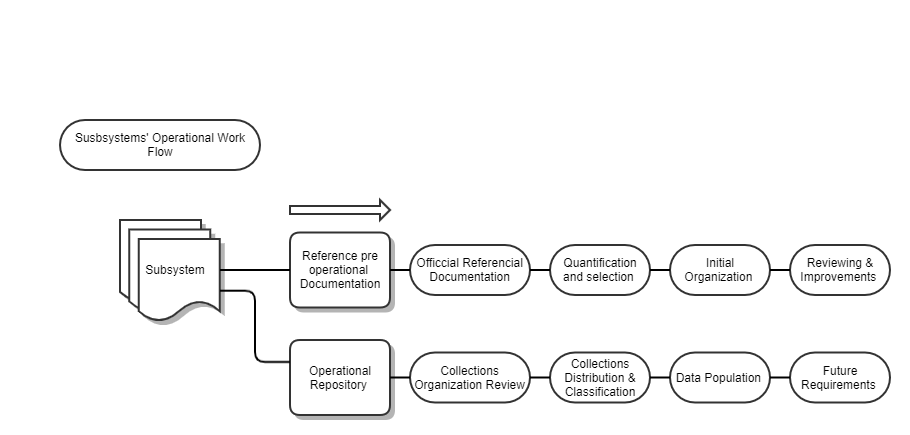
\includegraphics[width=\textwidth]{subsystems-role-workflow-temp}
\label{fig:subsystems-role-workflow}
\end{figure}

\begin{figure}[t]
\caption{Temporary Caption.}
\centering
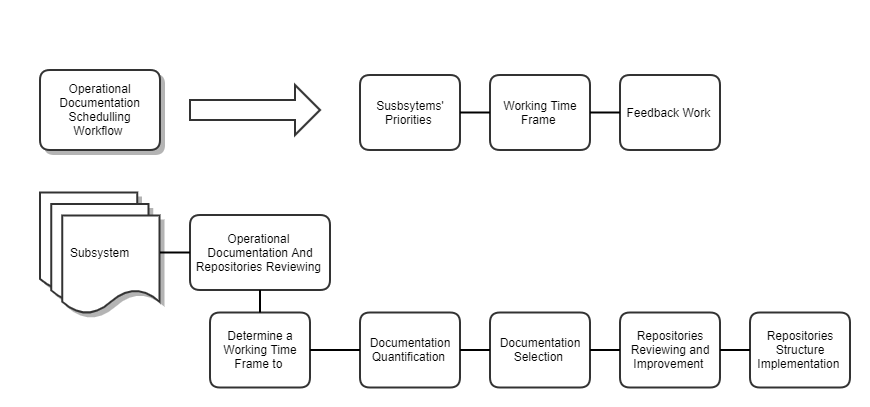
\includegraphics[width=\textwidth]{scheduling-workflow-temp}
\label{fig:scheduling-workflow}
\end{figure}
